\chapter{Paper Fighters}

We develop a multi-level-model based platformer called \textit{Paper Fighters}.
The user is able to design stages with the predefined components in Melanee's Model Editor and run them directly from the model, so he can play the stages or let other people play them. The following components are relevant for playing PaperFighters: the Melanee workbench with \textit{the Paper Painter plug-in} installed, which includes the Unity Application referred to as \textit{the Paper Fighters Client} and an implemented server socket, and a meta model illustrating the game architecture referred to as textit{the Paper Model}.
To create stages the user has to run Melanee with the plugin, and instansiate a PaperLevel into the Paper Model, which then several PaperStage objects can be added into. Subsequently a PaperFighter object representing the player has to be added to each stage, so it becomes playable. Afterwards as many components, as desired, except the player object due to the fact that it is (yet) a 1 Player game.
The plug-in simulates the deep model Paper Model, a LML file created in Melanee. Afterwards the simulation is passed to the Unity application which then instantiates the simulation. As soon as the state changes the Paper Fighters application sends the current state back to the model, where the changes in the game state are instantiated and updated in a lower level of our model, so the initial level does not get affected by our simulation.\\
The position of our PaperFighter object defines the start position of the player. The Aim is to get to a door
In the following sections the three main components and their contribution to Melanee are illustrated.

\section{The Paper Fighter Client}
The Paper Fighters Client is two dimensional platformer game implemented with the Unity game engine. It represents the simulation of our game. It consists of a Scene which represents the modeled stage. Relevant GameObjects contained by the scene are the NetworkClient-Objects, whose script implements the client socket and the StageManager-Object, which is referenced by the NetworkClient.

\subsection{The StageManager and NetworkClient}
The StageManager and Networ Client are GameObjects with a scripts attached. They have no visual representation and only serve functional purpose.
The StageManager is responsible for instatiating and destroying GameObjects and keeps track of their positions. It has refferrences of all predefined GameObjects and holds classes carrying the same attributes as the ones in our model. Moreover, it holds instances of these classes. The Player-Class which keeps track of the players position, has function to manipulate its type, position, size and speed. The Enemy-Class carries the same attributes as the player but has to be distinguishable due to the player position being dependent on the players input. To instantiate the StageComponents the class Box also holds type and positioning variables, as well a fix attribute which states whether the Rigidbody2D of our component is set to isKinematic. A StageComponent's position and size depends on the following four variables: fromX, fromY, toX and toY, which define a rectangle in our scene. The differences between our from and to variables determine their size. Because the StageComponents could rotate, in case their fix attribute is set to false, the position variable is set to be the centre of the calculated rectangle. Hence, even if the component rotates, our model is not informed, but will still continuously be aware of where the centre of our component lies. In addition, the described classes each have a toString() method attached, which converts the current state of the object into a string.
The StageManager also has a SimulationToModel() function, which enables capturing the current state of the current stage in form of a string.\\
The NetworkClient is a GameObject, which holds a script for networking purposes. It creates a client socket and starts communicating with the server as soon as our application is started.
Due to both GameObjects being part of two separate threads, we included a main thread dispatcher. This script is part of our a main thread and others can use it to push their events into its queue. By this, the main thread owning the script will consume them one after another. Our StageManager has one attached to receive the clients calls, without being interrupted. However, the StageManager has to send its state back to our client socket. This implies that our networking thread likewise needs a queue.\\
This entails, that our scene will have a little delay, and the pushed events will be handled asynchronously. On the other hand the calls received from our model will be executed chronologically.

\subsection{Stage Components}
All types of Stage Components from our model, except the hinge type, are Game Objects in the Unity contex. They have a script attached which allows them to define their size, their position in the game scene, calculating the borders of the collider. Depending on the attribute "isFix: Boolean",  whether they have a Rigidbody2D components attached or not. This component makes it possible to decide, whether a Stage Component reacts to gravity and can be impacted and moved by other game objects, or whether it is simply fixed, by using Unity's physics engine. Components with this attribute set to true can be used as ground. The attached colliders vary, depending on their "type: Character" attribute the Stage Component. For the "Rectangle"-type, it is a simple BoxCollider2D, which fits the rectangle, when the size is passed to the object. The “Line”-type has an EdgeCollider2D attached. The EdgeCollider2D takes start and end point of the line as nodes and creates an edge between them. Since Unity does not provide a collider for ellipses, the “Ellipse”-type also has an EdgeCollider2D attached. The corresponding script calculates its shape’s border, sets nodes around it, and creates edges along the nodes.
The Hinge Component represents the HingeJoint2D component in unity and is a component added to a GameObject. Thus, it has to have one GameObject as a bearer. The other optional one is then referenced inside the component by the objects Rigidbody2D. By setting the hinge's anchors it can be defined whether the object is fixated by a hinge
Each Player-GameObject has a script attached, which allows him/her to move according to the player’s input and, whose methods enable modification of its attributes like walking speed, jumping height, attack cool down, and size by scripts owned by other GameObjects. One instance of the Player-type is the "BlobNinja". His abilities are double jumping, throwing shurikens, and clinging to any objects having a collider. After clinging the double jump of our ninja is reset. The idle and walking animations each consist of two pictures, while the jump consists of three animations, depending on the vertical velocity the player object has. Depending on by what the player is hit there are different animations supported by triggering one of the following methods, "HandleBurnDamage()", "HandleLightningDamage()" or "HandleDamage()".\\
The Enemy-GameObject’s script provides similar modification functionality. Furthermore, each enemy type has an additional script, where different approaches in detecting and reacting to the Player-GameObject and movement behaviour is implemented.
The "FireGhost" is able to walk left and right until he detects a player. The speed it is moving with, and the time he needs to tun around can be set by accessing the attached script. Player detection is implemented in form of a circle. If the player enters it, the enemy starts moving into his direction and attacks him as soon as he is close.
"Zoys" is a floating character. While not detecting the player, he floats left and right similar to the FireGhost. The player detection is pretty much the same as well. The main difference is that he tries to position himself above the player and attacks from there with a fast lightning bolts. His collider is only where his body is, so the cloud he is attacking from is not hittable.
The Enemy-type "KungFrog" hops around in the same manner the other two enemy-types move. as soon as he detects the player. he jumps into his direction and shoots boxing gloves out of his mouth. As soon as the player comes too close, he tries to jump over him. While he is falling, the player can receive damage from touching him.

\section{Paper Painter Plug-in}

\begin{figure}
	\centering
	\includegraphics[scale=0.9]{grafiken/meltoolbar.jpg}
	\caption{Paper Painter Toolbar}
	\label{fig:4}
\end{figure}

\begin{figure}
	\centering
	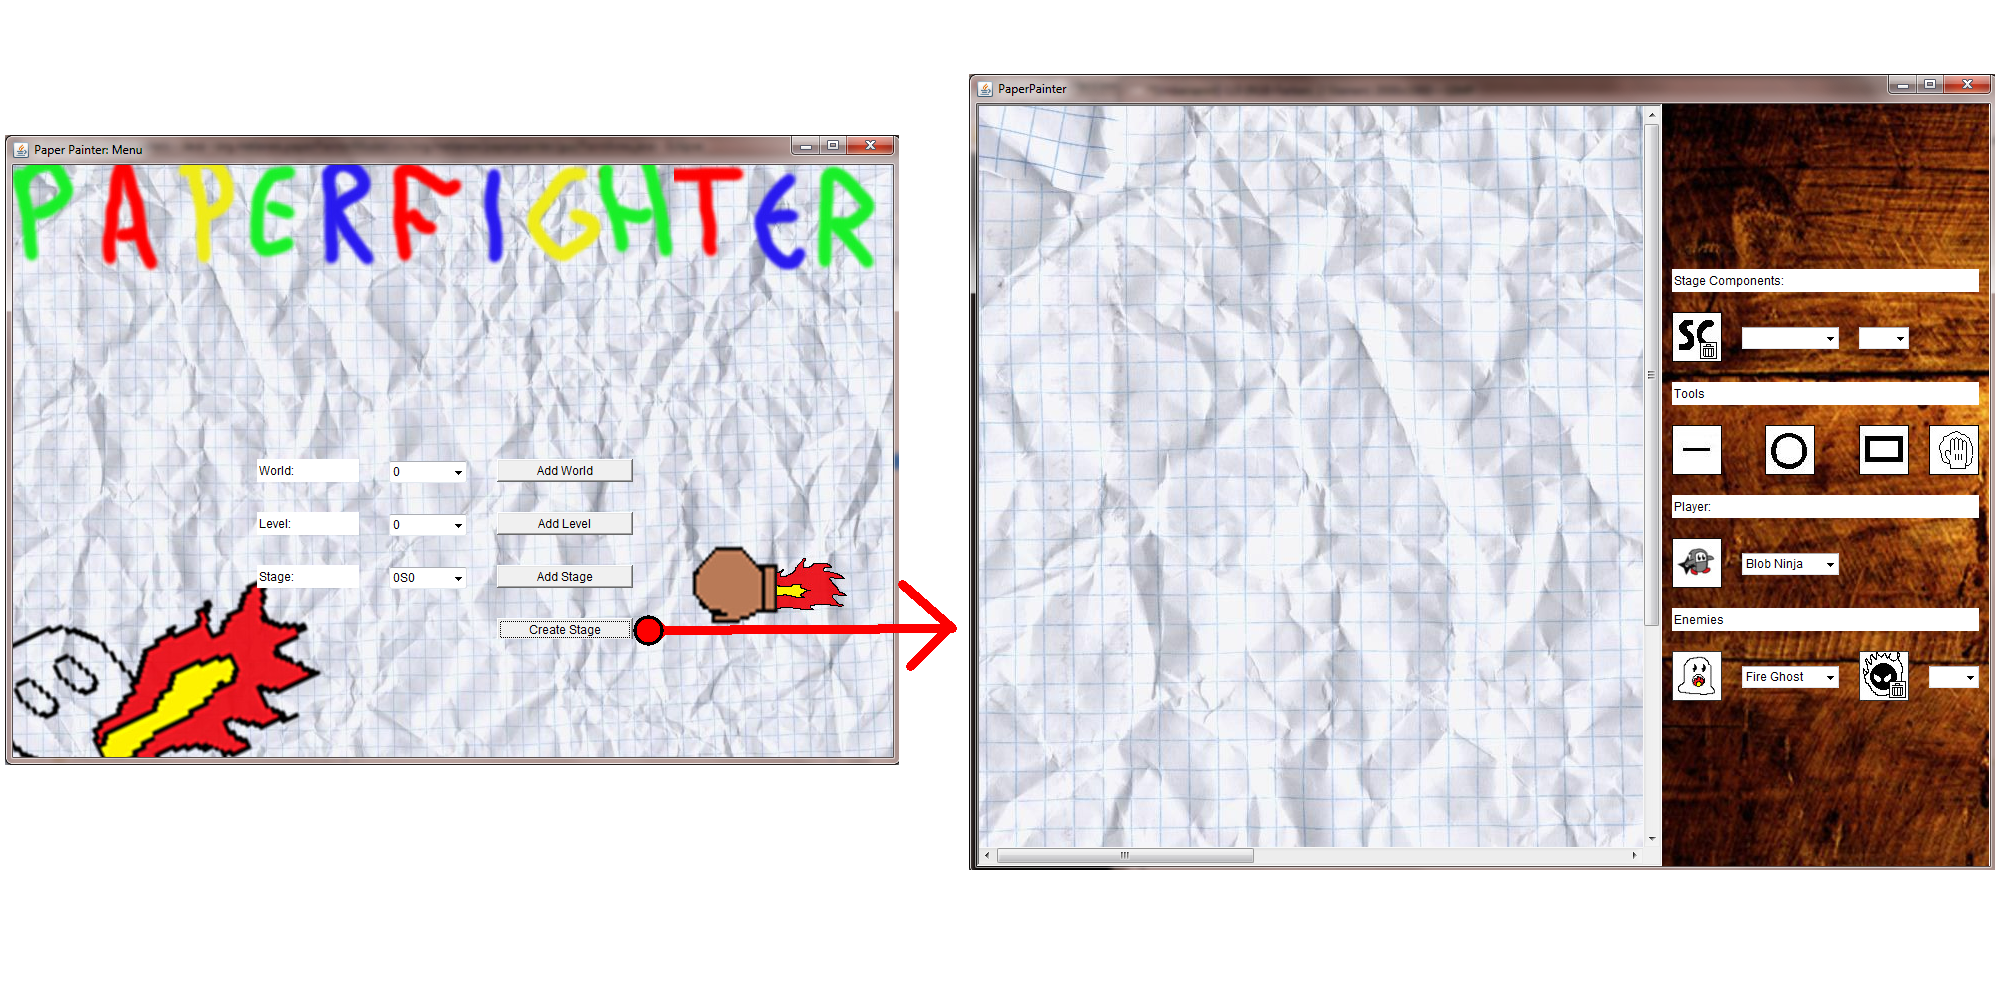
\includegraphics[scale=0.2]{grafiken/PaperPainter.png}
	\caption{Paper Painter GUI}
	\label{fig:5}
\end{figure}
We develop the Paper Painter plug-in for Melanee with the Eclipse PDE, which will be able to check the properties of an LML diagram, and to run an instance of our game if the entities' properties match our specifications. Hence, it provides modelling functionality for Paper Fighters. It uses the Melanee API to modify the deep model. The name of the created deep model must be “Paper Model“ and it has to consist of ontological levels with their names set to "O2 (Paper Model)" and "O3 (Paper Model)". As soon as these specifications are met, a Popup Bar appears in the mentioned levels with several buttons. For this purpose we extended our plug-in by the extension point org.melanee.workbench.popupbarbuttonprovider.provider. The two buttons "Let's Paint" and "Let's Play" can be observed in [Fig. \ref{fig:4}]. By pressing the "Let's Paint" button a frame implemented with the Abstract Widget Toolkit, opened, which can be observed in [Fig. \ref{fig:5}]. Within this frame instances of worlds which are a representation of a game, levels, and stages can be created. Stages are assigned to levels and levels are assigned to worlds to give a structure to one game. If the "Create Stage" button is pressed, another frame in which a painting application is implemented. With this free shapes, lines, rectangles and ellipses can be drawn. Moreover, the player-position can be set and enemies can be created and set to a desired position. The Frame instantiates them directly after they are painted holding their positions. Our Frame provides dropdown menus to select objects, declare if they are fix in the scene, and to select enemies in order to delete and reposition them. After closing the frame the objects will be passed to the corresponding stage. The "Let's Play" button creates a simulation out of our lml model and instantiates a server socket, which the simulation data is passed to. In addition it will start the Paper Fighter Client which connects with our server. Afterwards the client receives all modeled elements from the simulation as a string.
\\The plug-in is nested with classes which represent the game objects, and carry attributes corresponding to them. The classes attributes can all be modified, while the game is running via the model. The modification is then transmitted to the client, who will have to play the game with the recent modification. The Player.java, and Enemy.java classes define attributes for running speed, jumping height, size, and their position. A Box.java class defines shapes depending on its type attribute, which can be calculated inside a rectangle, like obviously rectangles, lines, and ellipses. Their position and size can also be modified during the game. Additionally, the attribute "isFix" can determine whether the object is considered as (higher) ground, or it is physically reacting to other objects, like other Box-, Enemy-, or Player-types. Furthermore, we described a FreeShape.java class which allows the modeling user to save freely painted pixels in the model, for this purpose the plug-in provides a PaperPainter.java, which is a GUI for drawing on the background and saving the drawn FreeShape- and Box-types, which both implement the interface IStageComponent.java in the PaperModel. Subsequently, we defined the class Hinge.java. It needs one and can hold up to two of type IStageComponents and has a position in the stage. When only one component is held, the component is pinned to the background at the hinges position and it can rotate around it, while when it holds two components, they are pinned to each other. By using one hinge for example on a line to pin it to the background, and another one to the line and a circle a pendulum can be modeled. The StageGoal.java class represents a way to another stage, or, if the "isLvlGoal" attribute is set, it represents the end of a level.
Representations for Stages, Levels, and Worlds are also implemented. A World contains Levels, a Level contains stages. The size of a certain Stage can be set by defining the "sizeX" and "sizeY" attributes. The background which is a A4 paper horizontally aligned is duplicated into the horizontal or vertical direction depending on the mentioned attributes. It's design was chosen to give the player the feeling to create a sketch and let it become alive. By this design different themes, like an ocean-, forest-, or volcano-theme can be retained through Levels which belong to the same world. This hierarchy is based on classical 2D platformer, which give the player the feeling of playing a story, whereby going on through the stages a kind of progress is conveyed.
\subsection{Server Socket}
As soon as the plug-in executes the unity client, it initializes a server socket and starts communicating with the client immediately. The plug-in starts three new threads, one for the server, another for receiving to messages and a third one for sending messages. Right now it is set for only one client, due to the fact that only one execution can be viewed in the model editor. Thereby the Melanee workbench will not get stopped during the communication. All classes are contained in the org.melanee.papermodel.traffic package. The code inside is provided by [\cite{SOC}]

\subsection{PaperSimulation}
The PaperSimulation.java class manages the entities of our execution model. With the "Let’s Play" button an instance of Simulation.java is instantiated and the modeled PaperLevel, its owned elements, and their properties are captured in . By getting all entities from the Paper Model our simulation creates objects from the corresponding classes contained by our plug-in.
Afterwards a server socket is initialized, and our UA is started. As soon as the UA is started, it instantiates a client socket that starts communicating with the server. When the connection is established the server sends the serialized byte stream to the client, so the created entities that match instances of our model in O1 can be created by the UA. Subsequently, the game starts sending its state back to the server as soon as something changes. The plug-in instantiates the execution state in O3, and starts updating it for each message.
The “Create Stage” button creates a new stage in the current PaperLevel context. In case, it is not the first one created, it creates a “source->next” connection to the last one created. The previous stage then becomes the source stage, and the freshly created becomes its next stage. Our simulation records the added stage and sends an update message to the UA.
Additionally, to the popup bar, our plug-in allows the user to define the position of all entities contained by a PaperStage by placing them at the desired position. As soon as the entity is placed, the position attributes are updated.
\section{Paper Model}
\begin{figure}
	\centering
	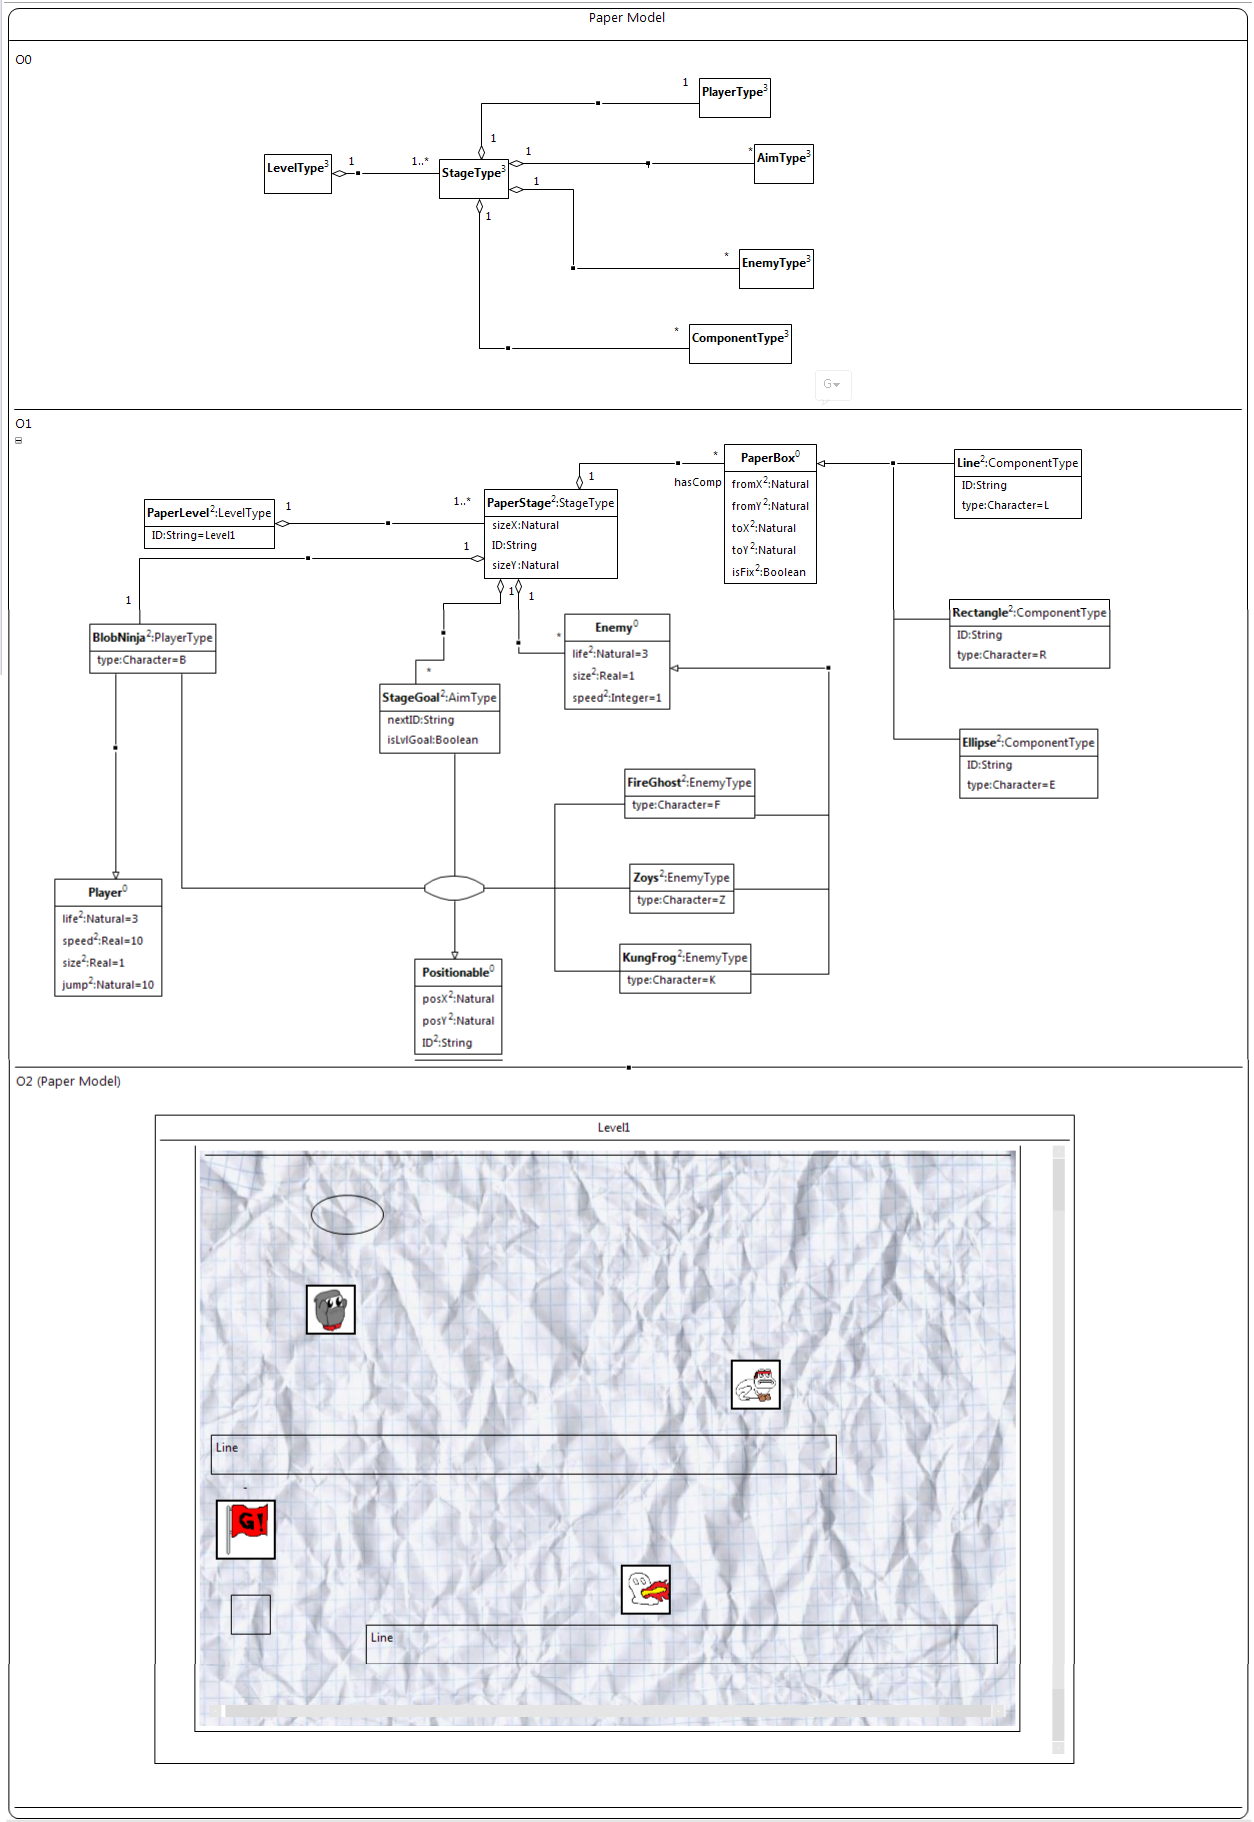
\includegraphics[scale=0.32]{grafiken/paperModel.png}
	\caption{The Paper Model}
	\label{fig:6}
\end{figure}
We create a LML diagram which represents the the model of our game by using Melanee's Model Editor. Inside the model we define the deep model \textit{Paper Model} illustrated in [Fig. \ref{fig:6}] which contains four ontological levels. "O0", defining and illustrating the modelling language, "O1", containing the actual model of our game, and "O2 (Paper Model)" which consists of an instance of the created PaperLevel.
The first level defines a modelling language for 2D platformers in general. Each game has one or more levels, where each is designed by retaining one theme to give the player the feel of a progressing story. A game level contains several stages, where one stage references other stages of the same level by adding their id to the StageGoal. By this reference it can be determined which stage can be reached from the current stage. This gives the player the feel of success, while coming closer to the last stage of the current level. Each stage contains one player, several enemies, several stage components, and one or more goals. By setting the goal’s attribute "isEnd: Boolean" the goal can be set as the end of our current level. The PlayerType is referenced by the stage, instead of the level. Hence, it is possible to set different PlayerTypes for different stages to challenge the player with different mechanics, while completing the level. The second level "O1" defines the model of Paper Fighters. It introduces its stage component types, and its enemy types. Furthermore, it shows the attributes of the stage objects. The attributes "posX: Natural" and "posY: Natural" of the differing stage objects like the player, enemies and stage goal, define their position inside the stage. In case of a PaperBox the attributes "fromX: Natural" and "fromY: Natural" define the position of the down left corner, and "toX: Natural" and "toY: Natural" define the position of the upright corner of a rectangle, in which it is instantiated. Instances of PaperFighter and PaperEnemy have additional attributes to modify their speed and size. By using Melanee’s graph-dsl plug-in we added visualization to each of the entities of "O1" instantiated in "O2", so each of their instances have a fitting visual representation in "O2 (Paper Model)".
After the initialization of the game all elements of "O2" are copied to a fourth level "O3 (Paper Model)", whose purpose is showing the execution state of the game, without having to change the initial level in "O2".